\documentclass{beamer}

\usepackage{algorithm}
\usepackage{algpseudocode}

\usepackage{listings}
\lstset{language=Python,keepspaces=true}
\usepackage{xcolor}

\lstset{
    basicstyle=\ttfamily\small,
    frame=single,
    breaklines=true,
    columns=fullflexible,
    showstringspaces=false
}

\newcommand{\R}{\mathbb{R}}  
\newcommand{\Z}{\mathbb{Z}}
\newcommand{\N}{\mathbb{N}}
\newcommand{\Q}{\mathbb{Q}}
\newcommand{\C}{\mathbb{C}}

% Theme and colors (Miami University style)
\usetheme{Madrid}
\usecolortheme{default}

\definecolor{MiamiRed}{RGB}{180,0,0}
\definecolor{MiamiWhite}{RGB}{255,255,255}
\setbeamercolor{structure}{fg=MiamiRed}
\setbeamercolor{frametitle}{bg=MiamiRed, fg=white}
\setbeamercolor{title}{fg=white, bg=MiamiRed}
\setbeamercolor{titlelike}{fg=white}
\setbeamercolor{block title}{bg=MiamiRed, fg=white}
\setbeamercolor{block body}{bg=gray!10, fg=black}

\makeatletter
\defbeamertemplate*{subsubsection page}{custom}{
  \begin{centering}
    \begin{beamercolorbox}[sep=8pt,center,rounded=true,shadow=false]{titlelike}
      \usebeamerfont{subsubsec} 
      \insertsection\par\vspace{0.2cm}
      \usebeamerfont{subsection title}\insertsubsection\par\vspace{0.2cm}
      \usebeamerfont{subsubsection title}\insertsubsubsection\par
    \end{beamercolorbox}
  \end{centering}
}
\newcommand{\subsubsectionpage}{\usebeamertemplate*{subsubsection page}}
\makeatother


\title{Traversing the Unlikely Intersection of Topological Data Analysis’s Mapper Algorithm and Pitch-Level MLB Data}
\author{Will Paz}
\date{\today}

\begin{document}

\frame{\titlepage}
%------------------------------------------------
\begin{frame}
    \frametitle{Outline}
    \tableofcontents
\end{frame}
%------------------------------------------------
\section{Introduction}
\begin{frame}
  \sectionpage
\end{frame}

%------------------------------------------------

%------------------------------------------------
\begin{frame}{Introduction}

\end{frame}

%------------------------------------------------
\begin{frame}{}

\end{frame}
%------------------------------------------------
\section{Toplogical Foundations}
\begin{frame}
  \sectionpage
\end{frame}

%------------------------------------------------
\begin{frame}{Topological Foundations}
\begin{block}{Definition}
    A topological space $(X, \tau)$ is a set $X$ equipped with a topology $\tau$, where $\tau$ is a collection of subsets of $X$, called open sets that satisfy the following conditions:
    \begin{enumerate}
        \item $\emptyset \in \tau$ and $X \in \tau$.
        \item $\tau$ is closed under arbitrary union, i.e. for any index set $A$ if $\{ U_\alpha \}_{\alpha \in A} \subseteq \tau$, then $\bigcup_{\alpha \in A} U_\alpha \in \tau$.
        \item $\tau$ is closed under finite intersection, i.e. if $U_1, U_2,...,U_n \in \tau$ then $\bigcap_{i=1}^n U_i \in \tau$.
    \end{enumerate}
\end{block}
\end{frame}
%------------------------------------------------
%------------------------------------------------
\begin{frame}{The Subspace Topology and Pairs}
\begin{block}{Definition}
    A subspace of a topological space $X$ is a subset $A \subset X$ equipped with the subspace topology $\tau_A$ defined by:
    \[
    \tau_A = \{ A \cap U : U \in \tau \}
    \]
\end{block}

\begin{block}{Definition}
    A pair of spaces $(X, A)$ is a space $X$ together with a subspace $A \subset X$. We can identify $X$ with the pair $(X,\emptyset)$. A pointed space is a pair $(X, \{x_0\}$). A map $f : (X, A) \to (Y, B)$ between pairs is a continuous function $f : X \to Y$ such that $f(A) \subset B$. Denote by $I = [0, 1]$ the unit interval.
\end{block}
\end{frame}
%------------------------------------------------
%------------------------------------------------
\begin{frame}{Introduction to Homotopy}
\begin{block}{Definition}
    Let $(X, A)$ be a pair and $f, g : X \to Y$ be two maps such that $f|_A$ = $g|_A$. Then we call $f$ homotopic to $g$ relative $A$ $(f \simeq g \operatorname{rel} A)$ if there exists a map 
    \[
    F : X \times I \to Y
    \]
    called homotopy such that $F(x, 0) = f(x)$ and $F(x, 1) = g(x)$ for all $x \in X$ and $F(x, t) = f(x) = g(x)$ for all $x \in A$ and $t \in I$. For $A = \emptyset$ we say $f$ is homotopic to $g$ ($f \simeq g$).
\end{block}

\begin{block}{Proposition}
    Homotopic relative $A$ is an equivalence relation on the set of maps.
\end{block}
\end{frame}
%------------------------------------------------
%------------------------------------------------
\begin{frame}{Homotopic Equivalence}
\begin{block}{Definition}
    Two spaces $X$ and $Y$ are called homotopy equivalent if there are maps $f : X \to Y$ and $g : Y \to X$ such that $gf \simeq \operatorname{id}_X$ and $fg \simeq \operatorname{id}_Y$. 
\end{block}
\begin{block}{Definition}
    A space is called contractible if it is homotopy equivalent to a one-point space.
\end{block}
\end{frame}
%------------------------------------------------
%------------------------------------------------
\begin{frame}{n-Simplices}
\begin{block}{Defintion}
    An $n$-simplex is a geometric object with $(n+1)$ vertices that lives in a $n$-dimensional space and cannot fit in any space of smaller dimension.
\end{block}
\begin{block}{Examples}
    \centering
    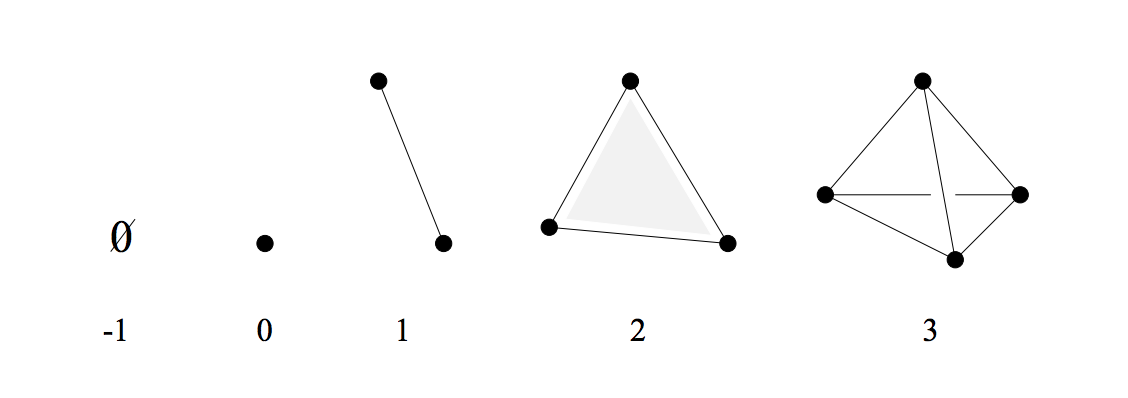
\includegraphics[width=0.7\linewidth]{Pictures/simplex.png}
\end{block}
\end{frame}
%------------------------------------------------
%------------------------------------------------
\begin{frame}{Simplicial Complexes}
\begin{block}{Definition}
    Let $\sigma = \langle x_0, .., x_n \rangle$ be a $n$-dimensional simplex. A face of $\sigma$ is a sub-simplex of $\sigma$ the simplex generated by a subset of vertices of $\sigma$. To get a face of $\sigma$ of dimension $m \leq n$, choose $m+1$ points among $x_0,...,x_n$ and take the corresponding simplex.
\end{block}

\begin{block}{Definition}
    A simplicial complex $K$ is a collection of simplices such that \begin{enumerate}
        \item If $K$ contains simplex $\sigma$, then $K$ also contains every face of $\sigma$.
        \item If two simplices of K intersect, then their intersection is a face of each of them.
    \end{enumerate}
\end{block}
\end{frame}
%------------------------------------------------

%------------------------------------------------
\begin{frame}{Nerve}
\begin{block}{Definition}
    Given a covering $\mathcal{U} = \{ U_\alpha \}_{\alpha \in A}$ of a topological space $X$, the nerve of the cover $\mathcal{U}$ denoted $N(\mathcal{U})$ is the simplicial complex whose vertex set corresponds to the index set $A$ with a finite subset $\{ \alpha_1,..., \alpha_n \} \subseteq A$ that span $(n-1)$ simplex in $N(\mathcal{U})$ if and only if $U_{\alpha_1} \cap \dots \cap U_{\alpha_n} \neq \emptyset$
\end{block}

\end{frame}
%------------------------------------------------

%------------------------------------------------
\begin{frame}{The Nerve Theorem}
\begin{block}{Theorem (The Nerve Theorem)}
    If $X$ is a topological space with a closed and convex covering $\mathcal{U}$, where each of the finite intersections of open sets are all contractable, then the nerve of the cover forms a simplicial complex that is homotopy equivalent to $X$, i.e. $X \simeq N(\mathcal{U})$.
\end{block}

\begin{block}{Note}
    The Nerve Theorem ensures that the topological graph constructed by overlapping preimages reflects the actual shape of the data, preserving connected components and loops.
\end{block}
\end{frame}
%------------------------------------------------

%------------------------------------------------
\begin{frame}{Reeb Graphs}
\begin{block}{Definition}
    Given a topological space $X$ and a continuous, real-valued function $f : X \to \mathbb{R}$, the Reeb Graph identifies the level set of $f$ at any value $c$ 

    \[
    f^{-1}(c) = \{x \in X : f(x) = c \}
    \]

    representing all points with the same function values.
\end{block}

\begin{block}{Note}
    A Reeb Graph is a continuous topological structure, where the Mapper algorithm is a discrete, data-driven approximation of it.
\end{block}
\end{frame}
%------------------------------------------------

%------------------------------------------------
\begin{frame}{Torus Example}
    \centering
    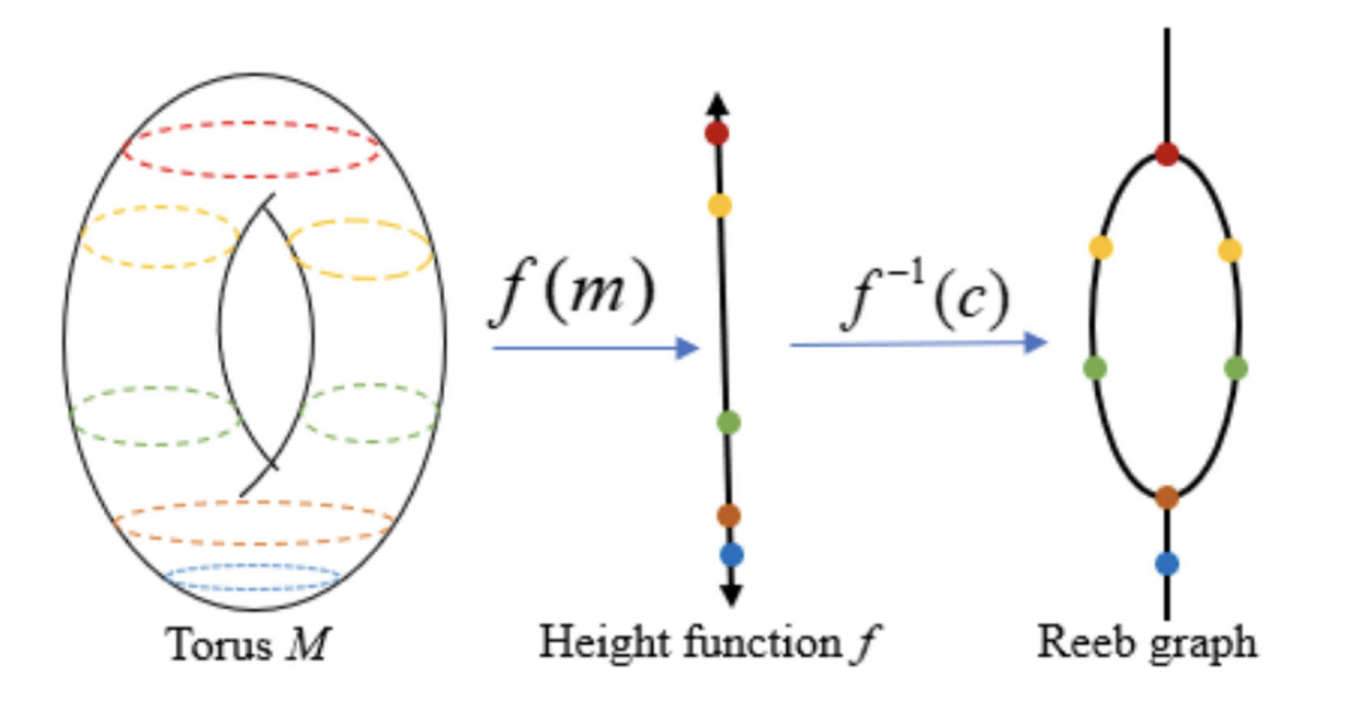
\includegraphics[width=0.9\linewidth]{Pictures/reeb_graph.png}
\end{frame}
%------------------------------------------------

%------------------------------------------------
\begin{frame}{Topological Graphs}
\begin{block}{Definition}
    Let $X$ and $X^*$ be topological spaces and $f : X \to X^*$ be a continuous map. Let $\mathcal{U} = \{ U_\alpha \}_{\alpha \in A}$ be a finite open set covering $X^*$ then consider \[
    f^*(\mathcal{U}) = \{ f^{-1} (U_\alpha) \}_{\alpha \in A},
    \]
    which is the covering of $X$ where $\{ f^{-1} (U_\alpha) \}_{\alpha \in A}$ is called the pullback of $\mathcal{U}$ along $f$. Then the topological graph $G$ is defined to be the nerve or the simplicial complex along index set $A$. We can write $G$ by:
    \[
    G(\mathcal{U}, f) = N(f^*(\mathcal{U})) = \left\{ \sigma \subseteq A : \bigcap_{\alpha \in \sigma} f^{-1} (U_\alpha) \neq \emptyset  \right\}
    \]
    where $\sigma$ represents a subset of the pullback cover $f^* (U_\alpha)$.
\end{block}
\end{frame}
%------------------------------------------------

%------------------------------------------------
\begin{frame}{Notes about Topological Graphs}
\begin{block}{Note}
    A collection of simplices $\sigma$ forms the nerve if the intersection of all preimages $f^{-1}(U_\alpha)$ for $\alpha \in \sigma$ is non-empty. In this context, the Mapper graph can be viewed as a discrete topological summary of $X$ induced by the continuous map $f$ reflecting its essential shape features.
\end{block}

\begin{block}{Note}
    In practice using real-valued point clouds, we must have a more statistical approach rooted in methods of dimensionality reduction, clustering, and a slew of relevant parameters.
\end{block}
\end{frame}
%------------------------------------------------

%------------------------------------------------
\section{The Mapper Algorithm}
\begin{frame}
  \sectionpage
\end{frame}

%------------------------------------------------

%------------------------------------------------
\begin{frame}{Overview}
\centering
    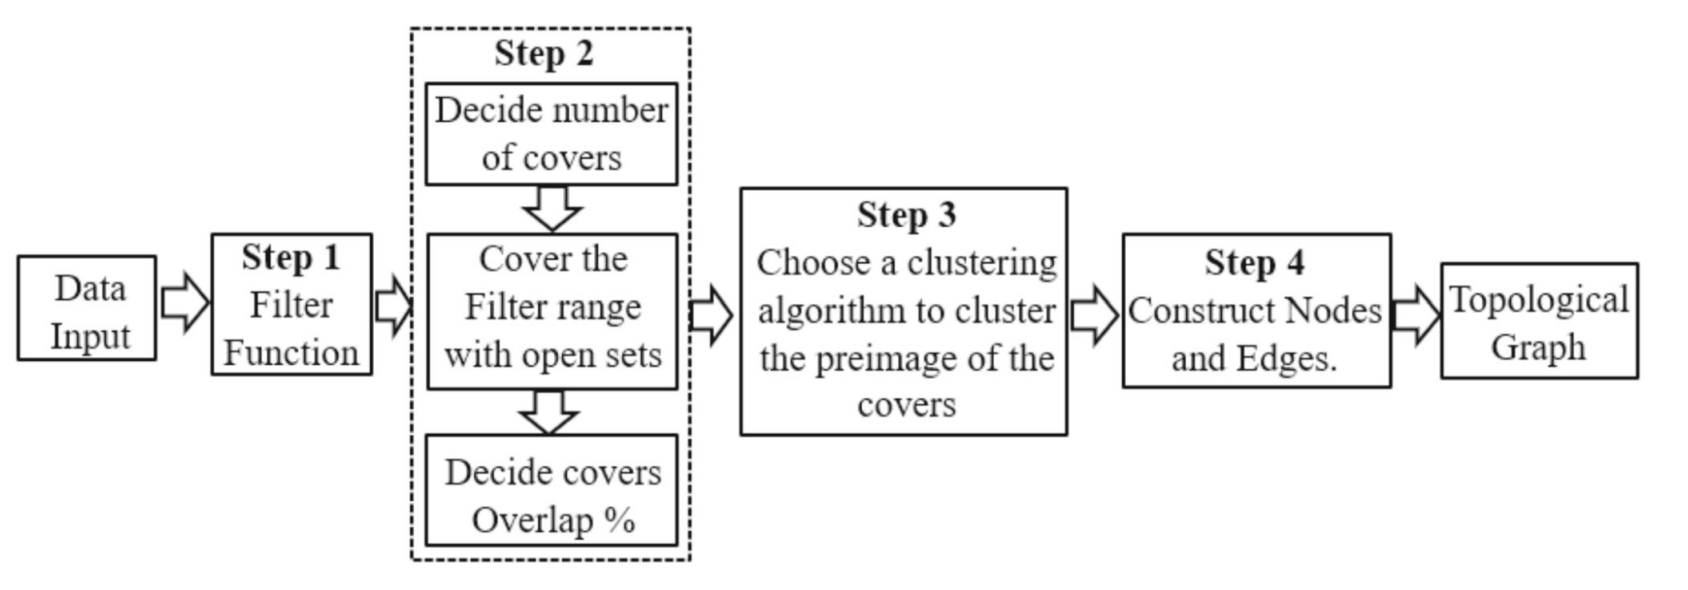
\includegraphics[width=1\linewidth]{Pictures/mapper_flow_chart.png}
\end{frame}
%------------------------------------------------

%------------------------------------------------
\subsection{Step 1: Choosing a Filter or Lens Function}
\begin{frame}
  \subsectionpage
\end{frame}

%------------------------------------------------

%------------------------------------------------
\begin{frame}{Step 1}
\begin{block}{Choosing a Filter or Lens Function}
    Given a high dimensional dataset $X \subset \mathbb{R}^n$, we can define a filter or lens function $f : X \to \mathbb{R}^k$ to reduce the dimension of the dataset to a lower Euclidean space $\mathbb{R}^k$, where $k < n$.
\end{block}

\begin{block}{Note}
    Selecting a dimension reduction method can vary by use cases based on the structure of the dataset. The most popular choice across TDA literature is Principal Component Analysis (PCA), and was chosen in this specific use case.
\end{block}
\end{frame}
%------------------------------------------------

%------------------------------------------------
\subsubsection{Principal Component Analysis (PCA)}
\begin{frame}
  \subsubsectionpage
\end{frame}

%------------------------------------------------


%------------------------------------------------
\begin{frame}{Principal Component Analysis (PCA)}
\begin{block}{Objective}
Principal Component Analysis (PCA) is defined as an orthogonal linear transformation to a lower-dimensional space that maximizes capturing explained variance in the project space. Where each coordinate corresponds to a principal component.
\end{block}

\begin{block}{Setup}
    Given a dataset with $m$ observations and $n$ features, we can construct a $m \times n$ matrix. For each feature/column, we must ensure the mean of the entries in the column is 0. Call this mean-centered matrix $\mathbf{A}$.
\end{block}
\end{frame}
%------------------------------------------------

%------------------------------------------------
\begin{frame}{Covariance Matrix}
\begin{block}{Covariance Matrix}
    We can define the sample covariance matrix of $\mathbf{A}$ to be
    \[
    Cov(\mathbf{A}) = \frac{1}{m-1}\mathbf{A}^T \mathbf{A}
    \]
    The diagonal entries of $Cov(\mathbf{A})$ are the variances of the individual features. The off-diagonal entries are the covariances between pairs of features.
\end{block}

\begin{block}{Note}
    Observe that $Cov(\mathbf{A}) \in \mathbb{R}^{n \times n}$ as is symmetric and positive semi-definite.
\end{block}
\end{frame}
%------------------------------------------------

%------------------------------------------------
\begin{frame}{The Spectral Theorem}
\begin{block}{The Spectral Theorem for Real, Symmetric Matricies}
    Consider a symmetric matrix $Cov(\mathbf{A}) \in \mathbb{R}^{n \times n}$. Then $Cov(\mathbf{A})$ has the following properties:
    \begin{enumerate}
        \item The eigenvalues of $Cov(\mathbf{A})$ are real.
        \item $Cov(\mathbf{A})$ is diagonalizable.
        \item There is a orthonormal basis of $\mathbb{R}^n$ consisting of eigenvectors of $Cov(\mathbf{A})$
    \end{enumerate}
    Therefore, $Cov(\mathbf{A})$ can be orthogonally diagonalized: $Cov(\mathbf{A}) = \mathbf{V}\mathbf{D}\mathbf{V}^T$, where $\mathbf{V} \in \mathbb{R}^{n \times n}$ is an orthonormal matrix of eigenvectors of $Cov(\mathbf{A})$, and $\mathbf{D} \in \mathbb{R}^{n \times n}$ is a real, diagonal matrix of eigenvalues of $Cov(\mathbf{A})$.
\end{block}
\end{frame}
%------------------------------------------------
%------------------------------------------------
\begin{frame}{PCA Notes}
\begin{block}{Observation}
See $\lambda_{\max}$ of the $Cov(\mathbf{A})$ corresponds to the largest variance of the dataset, and the associated eigenvector is the direction of maximum variance, called the first principal component.
\end{block}
\begin{block}{Note}
    In practice, PCA is never computer via explicit eigen-decomposition of $Cov(\mathbf{A})$ as it is numerically unstable for large $n$. Instead Singular Value Decomposition (SVD) is applied directly.
\end{block}
\end{frame}
%------------------------------------------------
%------------------------------------------------
\begin{frame}{Singular Value Decomposition}
\begin{block}{Theorem (Singular Value Decomposition)}
Suppose $\mathbf{A} \in \mathbb{R}^{m \times n}$ has $\text{rank}(\mathbf{A}) = n$, with $m \geq n$. Then we can write \[
\mathbf{A} = \mathbf{U} \mathbf{\Sigma} \mathbf{V}^T
\]
where the columns of $\mathbf{U} \in \mathbb{R}^{m \times m}$ and $\mathbf{V} \in \mathbb{R}^{n \times n}$, respectively, are orthonormal and $\mathbf{\Sigma} \in \mathbb{R}^{m \times n}$ is a diagonal matrix with entries $\sigma_i$ for $i = 1,...,n$, such that $\sigma_1 \geq \sigma_2 \geq \dots \geq \sigma_n \geq 0$. 
\end{block}
\begin{block}{Note}
We call $\{ \sigma_i\}_{i=1}^n$ the singular values of $\mathbf{A}$. We also call the columns of $\mathbf{U}$ the left singular vectors of $\mathbf{A}$, which are the eigenvectors of $\mathbf{A} \mathbf{A}^T$, and similarly call the columns of $\mathbf{V}$ the right singular vectors of $\mathbf{A}$, which are the eigenvectors of $\mathbf{A}^T \mathbf{A}$.
\end{block}
\end{frame}
%------------------------------------------------

%------------------------------------------------
\begin{frame}{Application of SVD}
\begin{block}{Key Fact}
The eigenvalues of $Cov(\mathbf{A})$ are precisely $\lambda_i = \frac{\sigma^2_i}{m-1}$.
\end{block}
\begin{block}{Key Idea}
Using SVD of $\mathbf{A}$, we can obtain the maximum variance as the largest squared singular value of $\mathbf{A}$, i.e. $\sigma^2_{1}$. We call the first principal component or the direction of maximum variance as the corresponding column of $\mathbf{V}$, call this associated eigenvector $v_1$.
\end{block}
\end{frame}
%------------------------------------------------

%------------------------------------------------
\begin{frame}{Partitioning}
\begin{block}{Observation}
Since $\mathbf{V}$ is an orthogonal matrix, then it follows that $\mathbf{A}\mathbf{V} = \mathbf{U} \mathbf{\Sigma}$.
\end{block}
\begin{block}{Proposition}
With our goal being to reduce dimensions to $\mathbb{R}^k$, where $k$ is the number of principal components, we should partition $\mathbf{V}$ into \[
\mathbf{V} = \left[  \mathbf{V}_k \ \ \mathbf{V}_\perp  \right]
\]
where $\mathbf{V}_k = [v_1  \dots v_k ] \in \mathbb{R}^{n \times k}$, and $v_1,...,v_k$ are the first $k$ principal directions.

\end{block}
\end{frame}
%------------------------------------------------

%------------------------------------------------
\begin{frame}{Projections}
\begin{block}{Proposition}
Define the projection map \[
\pi_k : \mathbb{R}^n \to \mathbb{R}^k
\]
where for any $x \in \mathbb{R}^n$, $z_i = \pi_k(x) = \mathbf{V}_k^T x$. The vector $z_i$ contains that observation's first $k$ principal-component scores. Therefore our data matrix is constructed to be $\mathbf{Z}_k = \mathbf{A} \mathbf{V}_k \in \mathbb{R}^{m \times k}$.
\end{block}
\begin{block}{Observation}
Given any $z_i \in \mathbf{Z}_k \subseteq \mathbb{R}^k$, we can find their approximation in original feature space by \[
a^*_i = \mathbf{V}_k z_i = \mathbf{V}_k \mathbf{V}_k^T x
\]
which is the best rank-$k$ approximation to $\mathbf{A}$ in squared-error or Frobenius-norm terms.
\end{block}
\end{frame}
%------------------------------------------------

%------------------------------------------------
\begin{frame}{Explained Variance}
\begin{block}{Definition}
Define the proportion of variance explained by component $j$ by \[
PVE_j = \frac{\lambda_j}{\sum_{l=1}^n \lambda_l} = \frac{\sigma_j^2}{\sum_{l =1}^n \sigma_l^2}
\]
\end{block}
\begin{block}{Definition}
Define the cumulative explained variance through component $j$ by \[
CVE_j = \frac{\sum_{l=1}^j \sigma_l^2}{\sum_{q=1}^n \sigma_q^2}
\]
\end{block}
\end{frame}
%------------------------------------------------

%------------------------------------------------
\begin{frame}{Selecting k}
\begin{block}{Reasoning}
The methods of looking at explained variance can give thresholds for how much variance we wish to allow for in our dimensionality reduction. Graphically, you can plot $\lambda_i$ versus $i$ and look for an "elbow." We use a two-dimensional PCA lens because it balances information retention, manageable cover complexity, and visual interpretability. 
\end{block}
\begin{block}{Limitations}
PCA provides a linear summary of these features. Nonlinear structure may remain, which motivates using Mapper to investigate the organization of the data beyond a purely linear model.
\end{block}
\end{frame}
%------------------------------------------------

%------------------------------------------------
\subsection{Step 2: Building a Cover}
\begin{frame}
  \subsectionpage
\end{frame}

%------------------------------------------------

%------------------------------------------------
\begin{frame}{Step 2}
\begin{block}{Building a Cover}
The next objective is to build a cover over the image of the projection map, $\pi_k(\mathbf{A})$, with the collection $\{ U_i \}_{i \in I}$, where $I$ is a finite indexing set. The set $\{ U_i \}_{i \in I}$ is composed of overlapping cubes (products of intervals).
\end{block}

\begin{block}{Parameterization}
In practice, values such as the number of cubes and percentage overlap between cubes are parameters given to the program. The amount of nodes and edges as well as the level of connectedness in the graph output is highly dependent on how these parameters are selected.
\end{block}
\end{frame}
%------------------------------------------------

%------------------------------------------------
\subsection{Step 3: Clustering}
\begin{frame}
  \subsectionpage
\end{frame}

%------------------------------------------------

%------------------------------------------------
\begin{frame}{Step 3}
\begin{block}{Clustering}
For each open set $U_i$ in the cover $\{ U_i \}_{i \in I}$, we want to cluster the points in the preimage $\pi_k^{-1}(U_i)$ to form a set of clusters $C_{i_q}$. There various clustering algorithms that could be used, but Density-Based Spatial Clustering of Applications with Noise (DBSCAN) was ultimately selected due to its popularity across application of the Mapper algorithm.
\end{block}
\end{frame}
%------------------------------------------------

%------------------------------------------------
\subsubsection{Density-Based Spatial Clustering of Applications with Noise (DBSCAN)}
\begin{frame}
  \subsubsectionpage
\end{frame}

%------------------------------------------------


%------------------------------------------------
\begin{frame}{Density Reachable}
\begin{block}{Definition}
Let the minimum elements allowed in any $\varepsilon$-neighborhood be called $M$. An element $x \in X$ is directly density-reachable from an element $y \in X$ with respect to $\varepsilon$ if \begin{enumerate}
    \item $x \in N_\varepsilon(y)$
    \item $|N_\varepsilon(y)| \geq M$
\end{enumerate}
\end{block}
\begin{block}{Definition}
An element $x \in X$ is density-reachable from an element $y \in X$ with respect to $\varepsilon$ and $M$ if there exists a chain of elements $x_1,..,x_n$, $x = x_1$, $x_n = y$, such that for all $1 \leq i \leq n-1$, $p_{i+1}$ is directly density reachable from $p_i$.
\end{block}
\end{frame}
%------------------------------------------------

%------------------------------------------------
\begin{frame}{Density Connectivity and Clusters}
\begin{block}{Definition}
An element $x \in X$ is density-connected to an element $y \in X$ with respect to $\varepsilon$ and $M$ if there exists a point $z \in X$ such that both $x$ and $y$ are density-reachable with respect to $\varepsilon$ and $M$.
\end{block}

\begin{block}{Definition}
Let $X$ be a point cloud holding our data. A cluster $C$ with respect to $\varepsilon$ and $M$ is a nonempty subset of $X$ satisfying the following conditions \begin{enumerate}
    \item For all $x,y \in X$, if $x \in C$ and $y$ is density-reachable with respect to $\varepsilon$ and $M$, then $y \in C$ (maximality)
    \item For all $x,y \in C$, $x$ is density-connected to $y$ with respect to $\varepsilon$ and $M$.
\end{enumerate}
\end{block}
\end{frame}
%------------------------------------------------

%------------------------------------------------
\begin{frame}{Noise and Uniqueness}
\begin{block}{Definition}
Let $C_1,...,C_k$ be the clusters of $X$ with respect to $\varepsilon_i$ and $M_i$, $i =1,...,k$. Then we define noise as the set of points in $X$ not belonging to any cluster, i.e. \[
\text{Noise} = \{ x \in X : \forall \ i, x \notin C_i \}
\]
\end{block}

\begin{block}{Lemma}
Let $C$ be a cluster with respect to $\varepsilon$ and $M$ and let $x \in C$ with $|N_\varepsilon(x)| \geq M$. Then \[
C = \{ y \in X : y \text{ is density reachable wrt $\varepsilon$ and $M$} \}
\]
\end{block}
\end{frame}
%------------------------------------------------

%------------------------------------------------
\begin{frame}{DBSCAN Algorithm}

\begin{block}{DBSCAN$(\textit{SetOfPoints}, \varepsilon, M)$}
\begin{algorithmic}[1]

\State \textbf{// Initially all points are UNCLASSIFIED}
\State $ClusterId \gets \textsc{NextId}(\textsc{NOISE})$

\For{$i \gets 1$ \textbf{to} $|\textit{SetOfPoints}|$}
    \State $Point \gets \textit{SetOfPoints}[i]$
    \If{$Point.ClId = \textsc{UNCLASSIFIED}$}
        \If{\Call{ExpandCluster}{$\textit{SetOfPoints}, Point, ClusterId, \varepsilon, M$}}
            \State $ClusterId \gets \textsc{NextId}(ClusterId)$
        \EndIf
    \EndIf
\EndFor

\end{algorithmic}
\end{block}

\end{frame}
%------------------------------------------------

%------------------------------------------------
\subsection{Step 4: Constructing the Mapper Topological Graph}
\begin{frame}
  \subsectionpage
\end{frame}

%------------------------------------------------

%------------------------------------------------
\begin{frame}{Building the Graph}
\begin{block}{Construction}
Each cluster $C_{i_q}$ forms a node $N$. And for any $i \leq j \leq I$, if clusters $C_{i_q}$ and $C_{j_p}$ have a nonempty intersection, then an edge $E$ is drawn connecting the two nodes; otherwise, singleton nodes are formed. This procedure yields our topological graph $G = (N,E)$.
\end{block}
\end{frame}
%------------------------------------------------

%------------------------------------------------
\subsection{KeplerMapper}
\begin{frame}
  \subsectionpage
\end{frame}

%------------------------------------------------

%------------------------------------------------
\begin{frame}{KeplerMapper}
\begin{block}{KeplerMapper}
\texttt{KeplerMapper} can be used for visualization of high-dimensional data and 3D point cloud data. \texttt{KeplerMapper} can make use of \texttt{Scikit-Learn} API compatible cluster and scaling algorithms. The package is a project found under the greater \texttt{scikit-tda} repository.
\end{block}

\centering
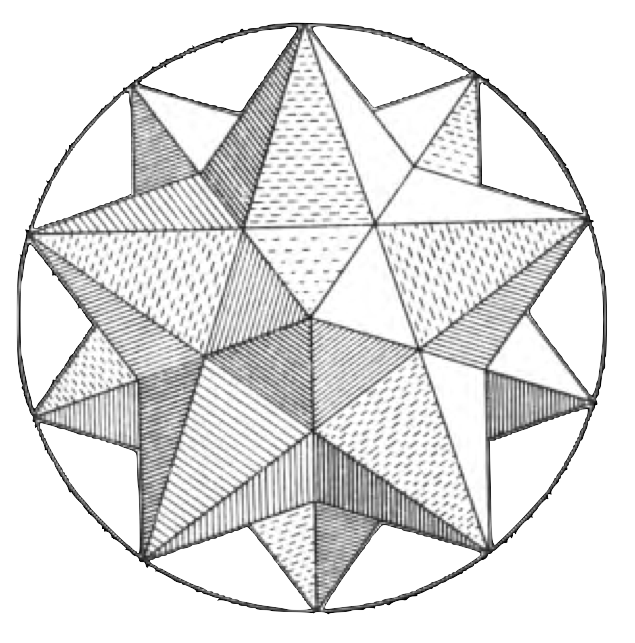
\includegraphics[width=0.5\linewidth]{Pictures/keplermapper.png}
\end{frame}
%------------------------------------------------

%------------------------------------------------
\begin{frame}[fragile]{KeplerMapper Code Block}
\begin{block}{Pseudo Code}
\leavevmode

\begin{lstlisting}[language=Python]
import kmapper as km
mapper = km.KeplerMapper()
lens = mapper.fit_transform(
    X,
    projection=PCA(n_components=2)
)
graph = mapper.map(
    lens,
    X,
    cover=km.Cover(
        n_cubes=10,
        perc_overlap=0.3
    ),
    clusterer=DBSCAN()
)
\end{lstlisting}
\end{block}
\end{frame}
%------------------------------------------------

%------------------------------------------------
\section{MLB Pitch-Level Data}
\begin{frame}
  \sectionpage
\end{frame}
%------------------------------------------------

%------------------------------------------------
\begin{frame}

\end{frame}
%------------------------------------------------

%------------------------------------------------
\begin{frame}

\end{frame}
%------------------------------------------------

%------------------------------------------------
\begin{frame}

\end{frame}
%------------------------------------------------

%------------------------------------------------
\begin{frame}

\end{frame}
%------------------------------------------------

%------------------------------------------------
\begin{frame}

\end{frame}
%------------------------------------------------

\end{document}